\section{饼图}

在这一节中,我们将学习如何使用D3来绘制饼图做数据可视化。我们会用到以下几个方法:

\begin{enumerate}
    \item SVG 路径:使用预定义的命令创建SVG路径
    \item \verb|d3.scaleOrdinal()|:创建序数比例尺
    \item \verb|d3.pie()|:饼图生成器
    \item \verb|d3.arc()|:弧生成器
\end{enumerate}

\subsection{SVG 路径}

路径元素用于在 SVG 上创建路径。我们可以使用命令在 SVG 中绘制出路径。 

\begin{minted}[frame=lines,framesep=2mm,baselinestretch=1.2,fontsize=\footnotesize,linenos]{html}
<body>
    <svg height="210" width="400">
        <path d="M150 0 L75 200 L225 200 Z" />
    </svg>
</body>
\end{minted}

如上述代码定义了一条从起点 (150, 0) 开始,经过 (75, 200), (225, 200) 的路径,并在起点处汇合。见\figref{fig:svg_path}所示。

\begin{figure}[htbp]
    \centering
    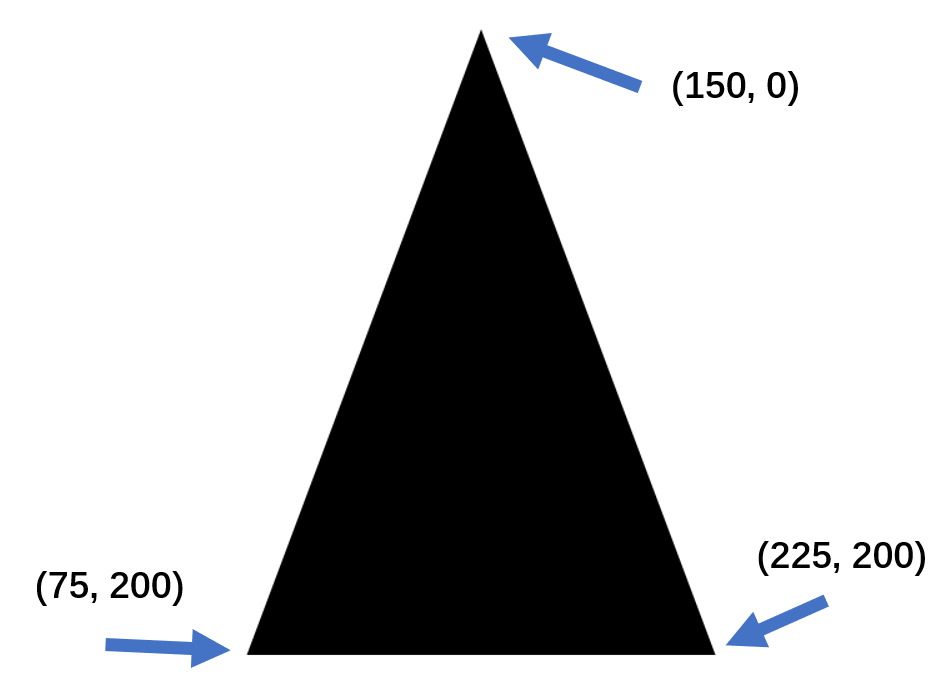
\includegraphics[width=0.6\textwidth]{figure/D3/svg_path.png}
    \caption{\textbf{SVG 路径}}
    \label{fig:svg_path}
\end{figure}

\subsection{d3.scaleOrdinal()}

我们在此前也学习过了比例尺的相关概念,此处我们会新使用到序数比例尺\verb|d3.scaleOrdinal()|。

\begin{minted}[frame=lines,framesep=2mm,baselinestretch=1.2,fontsize=\footnotesize,linenos]{html}
<script>
    var color = d3.scaleOrdinal(['#4daf4a','#377eb8','#ff7f00','#984ea3','#e41a1c']);
    console.log(color(0)) // #4daf4a
    console.log(color(1)) // #377eb8
    console.log(color(2)) // #ff7f00
    console.log(color(3)) // #984ea3
    console.log(color(4)) // #e41a1c
    console.log(color(5)) // #4daf4a,循环序数
</script>
\end{minted}

在这段代码中,我们定义了5种颜色,并进行了枚举遍历。当遍历到第6个值时,超出了颜色总数量会回到起点,即循环序数。

\subsection{d3.pie()}

\verb|d3.pie()|函数根据给定的数据,生成在SVG中的饼图对象(楔形)。对每一个楔形计算了初始角度和结束角度,而这便能被用于创建SVG中楔形的实际路径。

\begin{minted}[frame=lines,framesep=2mm,baselinestretch=1.2,fontsize=\footnotesize,linenos]{html}
<script>
    var data = [2, 4, 8, 10];
    var pie = d3.pie()
    console.log(pie(data))
</script>
\end{minted}

打开浏览器中的Console调试,可以看到log输出:

\begin{minted}[frame=lines,framesep=2mm,baselinestretch=1.2,fontsize=\footnotesize,linenos]{json}
[
    {
        "data": 2,
        "index": 3,
        "value": 2,
        "startAngle": 5.759586531581287,
        "endAngle": 6.283185307179586,
        "padAngle": 0
    },
    {...}, {...}, {...}
]
\end{minted}

\subsection{d3.arc()}

\verb|d3.arc()|函数生成弧,具体楔形的路径。弧需要一个内径和外径。如果内径为 0,则结果将是饼图,否则结果将是环形图。我们需要用到这些生成的弧线提供给我们的 SVG 路径元素。 

以下这段代码生成了一个简单的饼图,如\figref{fig:simple_pie}所示。

\begin{figure}[htbp]
    \centering
    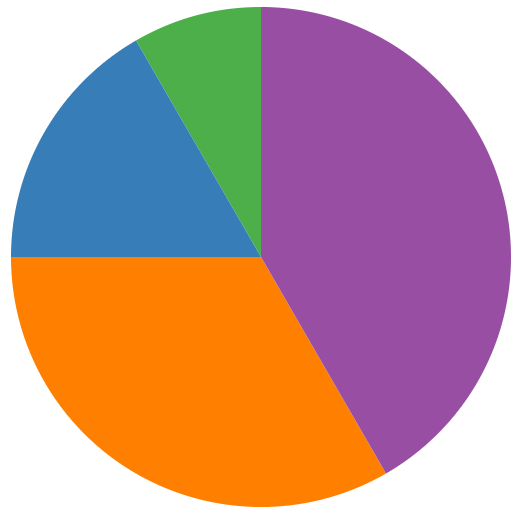
\includegraphics[width=0.5\textwidth]{figure/D3/simple_pie.png}
    \caption{\textbf{简单饼图}}
    \label{fig:simple_pie}
\end{figure}

\verb|<body>|标签内的部分:

\begin{minted}[frame=lines,framesep=2mm,baselinestretch=1.2,fontsize=\footnotesize,linenos]{html}
<body>
  <svg width="300" height="200"> </svg>
</body>
\end{minted}

\verb|<script>|脚本部分:

\begin{minted}[frame=lines,framesep=2mm,baselinestretch=1.2,fontsize=\footnotesize,linenos]{html}
<script>
  var data = [2, 4, 8, 10];

  // 定义宽 高 半径变量
  var svg = d3.select("svg"),
      width = svg.attr("width"),
      height = svg.attr("height"),
      radius = Math.min(width, height) / 2, // 保证不会超出SVG画布边界
      g = svg.append("g").attr("transform", "translate(" + width / 2 + "," + height / 2 + ")");
      // 添加组元素
  
  // 对颜色使用序数比例尺
  var color = d3.scaleOrdinal(['#4daf4a','#377eb8','#ff7f00','#984ea3','#e41a1c']);

  // 生成饼
  var pie = d3.pie();

  // 生成弧,设置内径和外径
  var arc = d3.arc()
              .innerRadius(0)
              .outerRadius(radius);

  // 生成组
  var arcs = g.selectAll("arc")
              .data(pie(data))
              .enter()
              .append("g")
              .attr("class", "arc")

  // 绘制路径,枚举序数填充颜色
  arcs.append("path")
      .attr("fill", function(d, i) {
          return color(i);
      })
      .attr("d", arc);
</script>
\end{minted}

\subsection{饼图案例:浏览器市场份额}

接下来,我们将以绘制桌面端浏览器市场份额饼图的实际案例来演示一个完整包含了标签等信息的饼图。

创建一个\verb|browser_share.csv|的CSV文件,内容为:

\begin{minted}[frame=lines,framesep=2mm,baselinestretch=1.2,fontsize=\footnotesize,linenos]{html}
browser,percent
Chrome,68.4
Safari,9.41
Firefox,8.03
Edge,6.36
Opera,2.5
其他,5.3
\end{minted}

完整代码如下,绘制出的效果如\figref{fig:pie_browser_share}所示。

\begin{figure}[htbp]
    \centering
    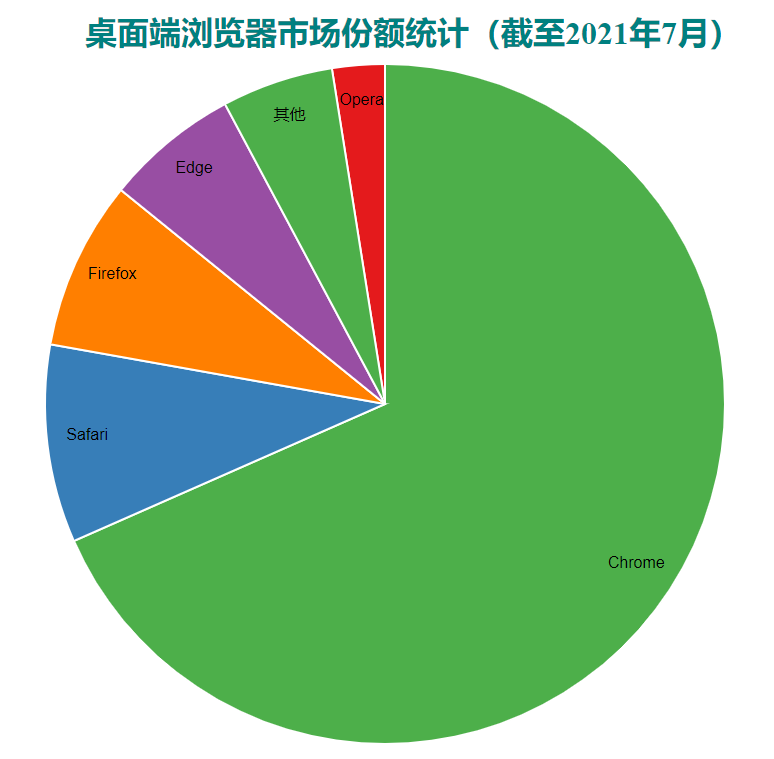
\includegraphics[width=0.7\textwidth]{figure/D3/pie_browser_share.png}
    \caption{\textbf{桌面端浏览器市场份额统计(截至2021年7月)}}
    \label{fig:pie_browser_share}
\end{figure}

\begin{minted}[frame=lines,framesep=2mm,baselinestretch=1.2,fontsize=\footnotesize,linenos]{html}
<!DOCTYPE html>
<html lang="en">
  <head>
    <meta charset="UTF-8" />
    <meta name="viewport" content="width=device-width, initial-scale=1.0" />
    <title>D3.js</title>

    <!-- 引入D3 -->
    <script src="./js/d3.min.js" charset="utf-8"></script>
  </head>
  <body>
    <svg width="500" height="400"></svg>
  </body>
</html>

<script>
  var svg = d3.select("svg"),
    width = svg.attr("width"),
    height = svg.attr("height"),
    radius = Math.min(width, height) / 2;

  var g = svg
    .append("g")
    .attr("transform", "translate(" + width / 2 + "," + height / 2 + ")");

  var color = d3.scaleOrdinal([
    "#4daf4a",
    "#377eb8",
    "#ff7f00",
    "#984ea3",
    "#e41a1c",
  ]);

  // 创建匿名函数返回数据中百分比的值
  var pie = d3.pie().value(function (d) {
    return d.percent;
  });

  // 定义内径和外径
  var arc = d3
    .arc()
    .outerRadius(radius - 30)
    .innerRadius(90); // 0时为饼图,非0为环形图

  // 定义标签所在位置
  var label = d3
    .arc()
    .outerRadius(radius)
    .innerRadius(radius - 100);

  // 读取 CSV 文件
  d3.csv("browser_share.csv").then(function (data) {
    // 为每个data创建组元素
    var arcs = g
      .selectAll(".arc")
      .data(pie(data))
      .enter()
      .append("g")
      .attr("class", "arc");

    // 将路径元素添加进组中
    // 使用序数比例尺填充颜色
    arcs
      .append("path")
      .attr("d", arc)
      .attr("fill", function (d) {
        return color(d.data.browser);
      });
    
    // 在每个楔形中填写标签为浏览器名
    arcs
      .append("text")
      .attr("transform", function (d) {
        return "translate(" + label.centroid(d) + ")";
      })
      .text(function (d) {
        return d.data.browser;
      });
  });

  // 添加图表标题
  svg
    .append("g")
    .attr("transform", "translate(" + (width / 2 - 150) + "," + 20 + ")")
    .append("text")
    .text("桌面端浏览器市场份额统计(截至2021年7月)")
    .attr("class", "title");
</script>

<style>
  /* 设置 CSS 样式 */
  .arc text {
    font: 8px sans-serif;
    text-anchor: middle;
  }

  .arc path {
    stroke: #fff;
  }

  .title {
    fill: teal;
    font-weight: bold;
  }
</style>
\end{minted}

若在为\verb|arc|设置内径时,不为0,如设置成90则可得到环形图,如\figref{fig:donut_browser_share}所示。

\begin{figure}[htbp]
    \centering
    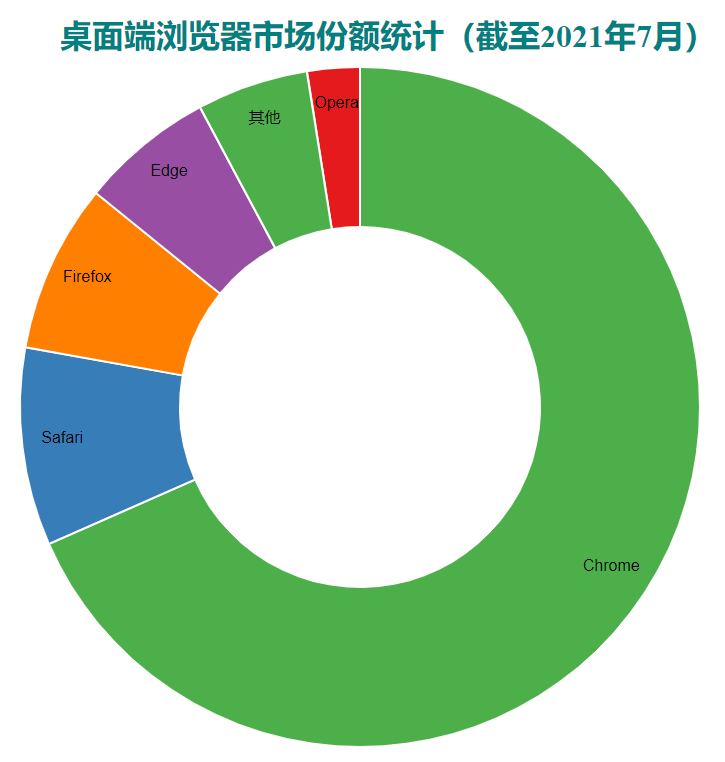
\includegraphics[width=0.7\textwidth]{figure/D3/donut_browser_share.png}
    \caption{\textbf{环形图}}
    \label{fig:donut_browser_share}
\end{figure}